%%%--------------------------------%%%
%%% Implementation
%%%--------------------------------%%%

\section{Design Approach}
\label{sec:implementationDesign}

As can be seen in the screenshots in this chapter, the application makes use of analogous colors, so colors that are similar to each other. The authors decided to choose green- and blue shades as they appear to be calming towards the application users which is intended to be helpful in the unpleasant context of discussing problematic risks.

Besides the similar looking colors, the application is build with reusable atomic third-party components like buttons or form fields. This leads on one hand to accelerated development of the application due to the ready-made components, but on the other hand to simplification in terms of usability as the users can be sure that the components will look and behave the same way in every part of the application.

On top of that, due to the surveys feedback, the application was development with multiple platforms in mind (\ref{sec:DomainAa}). Those polled would like to use the application on mobile and desktop devices which is why the approach of a  \acs{PWA} (\ref{sec:theorieCa}) was adhered to. The resulting application now fulfills various criteria of a PWA. It is progressive and re-engagable by using notifications if desired (\ref{sec:theorieCa}. Some parts are network independent and cache the servers result, HTTPS is already used in development and due to a provided service worker and manifest the application is discoverable, installable and linkable. Figure \ref{fig:activitystreamcombined} shows the activity stream on desktop and mobile to demonstrate the responsiveness which is also a realized criterion of a  \acs{PWA}.

\begin{figure}[H]
	\centering
	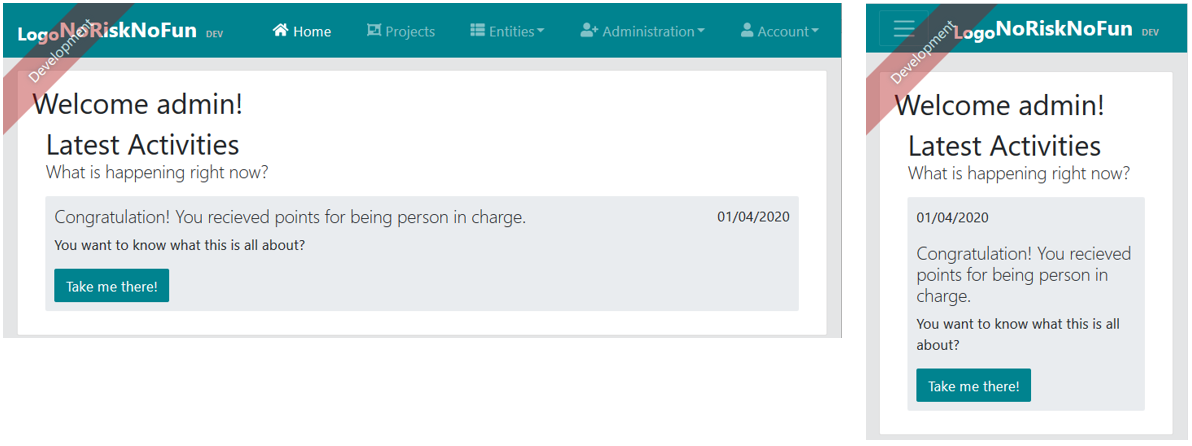
\includegraphics[width=0.8\textwidth]{Assets/implementation_shots/activitystreamcombined.png}
	\caption{Screenshot comparing desktop and mobile view}
	\label{fig:activitystreamcombined}
\end{figure}

In the further development, the application could be improved by providing a more comprehensive caching of server results and better responsiveness in various parts of the application.
